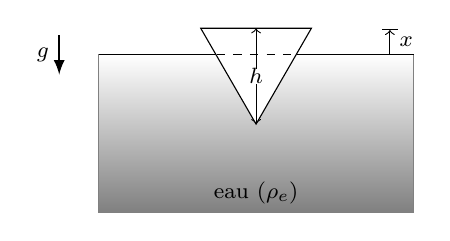
\begin{tikzpicture} [
	scale=1,
	font=\footnotesize,
	vecteur/.style={-latex,thick},
	]
	% liquide
	\shadedraw[color=gray,top color=white,bottom color=gray] (-2,0)--++(4,0)--++(0,-2)--++(-4,0)--cycle;
	\draw (-2,0)--++(4,0);
	\draw (0,-1.75) node{eau ($\rho_\text{e}$)};
	% solide
	\draw[fill=white,shift={(0,-25pt)}](0,0)--(120:40pt)--++(0:40pt)--cycle;
	\draw[dashed,thin] (-.5,0)--++(1,0);
	\draw[shift={(0,-25pt)},<->](0,0)--++(0,34.6pt)node[inner sep=0,midway,fill=white]{$h$};
	\draw[->|](1.7,0)--++(0,9.4pt)node[midway,right]{$x$};
	% forces
	\draw[vecteur] (-2.5,0.25)--++(0,-0.5) node[pos=0.5,left]{$\vv{g}$};
	% \draw[help lines] (-2,-2) grid (2,2);
\end{tikzpicture}